% Options for packages loaded elsewhere
\PassOptionsToPackage{unicode}{hyperref}
\PassOptionsToPackage{hyphens}{url}
%
\documentclass[
]{article}
\usepackage{lmodern}
\usepackage{amsmath}
\usepackage{ifxetex,ifluatex}
\ifnum 0\ifxetex 1\fi\ifluatex 1\fi=0 % if pdftex
  \usepackage[T1]{fontenc}
  \usepackage[utf8]{inputenc}
  \usepackage{textcomp} % provide euro and other symbols
  \usepackage{amssymb}
\else % if luatex or xetex
  \usepackage{unicode-math}
  \defaultfontfeatures{Scale=MatchLowercase}
  \defaultfontfeatures[\rmfamily]{Ligatures=TeX,Scale=1}
\fi
% Use upquote if available, for straight quotes in verbatim environments
\IfFileExists{upquote.sty}{\usepackage{upquote}}{}
\IfFileExists{microtype.sty}{% use microtype if available
  \usepackage[]{microtype}
  \UseMicrotypeSet[protrusion]{basicmath} % disable protrusion for tt fonts
}{}
\makeatletter
\@ifundefined{KOMAClassName}{% if non-KOMA class
  \IfFileExists{parskip.sty}{%
    \usepackage{parskip}
  }{% else
    \setlength{\parindent}{0pt}
    \setlength{\parskip}{6pt plus 2pt minus 1pt}}
}{% if KOMA class
  \KOMAoptions{parskip=half}}
\makeatother
\usepackage{xcolor}
\IfFileExists{xurl.sty}{\usepackage{xurl}}{} % add URL line breaks if available
\IfFileExists{bookmark.sty}{\usepackage{bookmark}}{\usepackage{hyperref}}
\hypersetup{
  pdftitle={Comparison of Ensemble Recalibration Methods in Flu Forecasting},
  pdfauthor={Nutcha Wattanachit},
  hidelinks,
  pdfcreator={LaTeX via pandoc}}
\urlstyle{same} % disable monospaced font for URLs
\usepackage[margin=1in]{geometry}
\usepackage{graphicx}
\makeatletter
\def\maxwidth{\ifdim\Gin@nat@width>\linewidth\linewidth\else\Gin@nat@width\fi}
\def\maxheight{\ifdim\Gin@nat@height>\textheight\textheight\else\Gin@nat@height\fi}
\makeatother
% Scale images if necessary, so that they will not overflow the page
% margins by default, and it is still possible to overwrite the defaults
% using explicit options in \includegraphics[width, height, ...]{}
\setkeys{Gin}{width=\maxwidth,height=\maxheight,keepaspectratio}
% Set default figure placement to htbp
\makeatletter
\def\fps@figure{htbp}
\makeatother
\setlength{\emergencystretch}{3em} % prevent overfull lines
\providecommand{\tightlist}{%
  \setlength{\itemsep}{0pt}\setlength{\parskip}{0pt}}
\setcounter{secnumdepth}{-\maxdimen} % remove section numbering
\usepackage{booktabs}
\usepackage[utf8]{inputenc}
\usepackage{tabularx}
\usepackage{amsmath}
\usepackage{amssymb}
\usepackage{hyperref}
\usepackage{multicol}
\usepackage{longtable}
\usepackage{array}
\usepackage{multirow}
\usepackage{wrapfig}
\usepackage{float}
\usepackage{colortbl}
\usepackage{pdflscape}
\usepackage{tabu}
\usepackage{threeparttable}
\usepackage{threeparttablex}
\usepackage{makecell}
\usepackage{xcolor}
\usepackage{float}
\usepackage{booktabs}
\usepackage{longtable}
\usepackage{array}
\usepackage{multirow}
\usepackage{wrapfig}
\usepackage{colortbl}
\usepackage{pdflscape}
\usepackage{tabu}
\usepackage{threeparttable}
\usepackage{threeparttablex}
\usepackage[normalem]{ulem}
\usepackage{makecell}
\usepackage{xcolor}
\ifluatex
  \usepackage{selnolig}  % disable illegal ligatures
\fi

\title{Comparison of Ensemble Recalibration Methods in Flu Forecasting}
\author{Nutcha Wattanachit}
\date{12/14/2020}

\begin{document}
\maketitle

We compare 1) the equally-weighted ensemble, 2) the traditional linear
pool (TLP), 3) the beta-transform linear pool (BLP), 4) the
equally-weighted beta-transform linear pool, 5) the Bayesian finite beta
mixture 6) the Bayesian finite beta mixture with equally-weighted
component forecasts in the simulation studies and in the application of
influenza forecasting. For both beta mixture approaches, the number of
mixing beta components are \(K=2,3,\) and \(4\).

\hypertarget{methods}{%
\section{Methods}\label{methods}}

Let \(f_1,...,f_M\) be predictive density forecasts from \(M\) component
forecasting models, the ensemble methods combine the component
forecasting models as follows

\hypertarget{equally-weighted-ensemble-ew}{%
\subsection{Equally-weighted ensemble
(EW)}\label{equally-weighted-ensemble-ew}}

The equally-weighted ensemble combines the component forecasting models
with the aggregation predictive distribution function

\begin{align}
f_{\text{EW}}(y)=\sum_{m=1}^M \frac{1}{M}f_m(y).
\end{align}

\hypertarget{traditional-linear-pool-tlp}{%
\subsection{Traditional linear pool
(TLP)}\label{traditional-linear-pool-tlp}}

The TLP finds a set of optimal nonnegative weights \(w_i\) that maximize
the likelihood of the aggregation predictive distribution function

\begin{align}
f_{\text{TLP}}(y)=\sum_{m=1}^M w_mf_m(y),
\end{align}

where \(\sum_{m=1}^M w_m=1\). The TLP is underdispersed when the
component models are probabilistically calibrated.

\hypertarget{beta-transform-linear-pool-blp}{%
\subsection{Beta-transform linear pool
(BLP)}\label{beta-transform-linear-pool-blp}}

The BLP applies a beta transform on the combined predictive cumulative
distribution function

\begin{align}
F_{\text{BLP}}(y)=B_{\alpha,\beta}\Big(\sum_{m=1}^M w_m F_m(y)\Big),
\end{align}

Specifically, the BLP finds the transformation parameters
\(\alpha,\beta > 0\), and a set of nonnegative weights \(w_m\) that
maximize the likelihood of the aggregated predictive distribution
function

\begin{align}
f_{\text{BLP}}(y)=\Big(\sum_{m=1}^M w_mf_m(y)\Big)b_{\alpha,\beta}\Big(\sum_{m=1}^M w_m F_m(y)\Big),
\end{align}

where \(b_{\alpha,\beta}\) denotes the beta density and
\(\sum_{m=1}^M w_m=1\).

\hypertarget{equally-weighted-beta-transform-linear-pool-ew-blp}{%
\subsection{Equally-weighted beta-transform linear pool
(EW-BLP)}\label{equally-weighted-beta-transform-linear-pool-ew-blp}}

The EW-BLP applies a beta transform on the equally-weighted ensemble and
has the predictive cumulative distribution function

\begin{align}
F_{\text{EW-BLP}}(y)=B_{\alpha,\beta}\Big(\sum_{m=1}^M \frac{1}{M} F_m(y)\Big),
\end{align}

The EW-BLP finds the transformation parameters \(\alpha,\beta > 0\) that
maximize the likelihood of the aggregated predictive distribution
function

\begin{align}
f_{\text{EW-BLP}}(y)=\Big(\sum_{m=1}^M w_mf_m(y)\Big)b_{\alpha,\beta}\Big(\sum_{m=1}^M \frac{1}{M} F_m(y)\Big).
\end{align}

\hypertarget{bayesian-finite-beta-mixture-textbm_k}{%
\subsection{\texorpdfstring{Bayesian finite beta mixture
(\(\text{BM}_k\))}{Bayesian finite beta mixture (\textbackslash text\{BM\}\_k)}}\label{bayesian-finite-beta-mixture-textbm_k}}

The \(\text{BM}_k\) extends the BLP method by using a finite beta
mixture combination formula

\begin{align}
F_{\text{BM}_k}(y)=\sum_{k=1}^K w_kB_{\alpha,\beta}\Big(\sum_{m=1}^M \omega_{km} F_m(y)\Big),
\end{align}

where the vector \(w_1,..., w_K\) comprises the beta mixture weights,
\(\alpha_1,..., \alpha_K\) and \(\beta_1,..., \beta_K\) are beta
calibration parameters, and for each beta component
\(\boldsymbol{\omega}_k=(\omega_{k1},..., \omega_{kM})\) comprises the
beta component-specific set of component model weights. The pdf
representation of the method is

\begin{align}
f_{\text{BM}_k}(y)=\sum_{k=1}^K w_k(\sum_{m=1}^M \omega_{km} f_m(y)\Big)b_{\alpha,\beta}\Big(\sum_{m=1}^M \omega_{km} F_m(y)\Big).
\end{align}

\hypertarget{bayesian-finite-equally-weighted-beta-mixture-textew-bm_k}{%
\subsection{\texorpdfstring{Bayesian finite equally weighted beta
mixture
(\(\text{EW-BM}_k\))}{Bayesian finite equally weighted beta mixture (\textbackslash text\{EW-BM\}\_k)}}\label{bayesian-finite-equally-weighted-beta-mixture-textew-bm_k}}

The \(\text{EW-BM}_k\) uses a finite beta mixture combination formula to
combine an equally-weighted ensemble as follows

\begin{align}
F_{\text{EW-BM}_k}(y)=\sum_{k=1}^K w_kB_{\alpha,\beta}\Big(\sum_{m=1}^M \frac{1}{M} F_m(y)\Big),
\end{align}

where the vector \(w_1,..., w_K\) comprises the beta mixture weights and
\(\alpha_1,..., \alpha_K\) and \(\beta_1,..., \beta_K\) are beta
calibration parameters.

\begin{align}
f_{\text{EW-BM}_k}(y)=\sum_{k=1}^K w_k(\sum_{m=1}^M \frac{1}{M} f_m(y)\Big)b_{\alpha,\beta}\Big(\sum_{m=1}^M \frac{1}{M} F_m(y)\Big).
\end{align}

\hypertarget{simulation-studies}{%
\section{Simulation studies}\label{simulation-studies}}

\hypertarget{scenario-1-unbiased-and-calibrated-components}{%
\subsection{Scenario 1: Unbiased and calibrated
components}\label{scenario-1-unbiased-and-calibrated-components}}

The data generating process for the observation \(Y\) in the regression
model is

\[
Y = X_0+a_1X_1+a_2X_2+a_3X_3+ \epsilon, \\
\epsilon \sim N(0,1)
\] where \(a_1=1,a_2=1,\) and \(a_3=1.1\), and \(X_0,X_1,X_2,X_3,\) and
\(\epsilon\) are independent, standard normal random variables. The
TLP's PITs are approximately beta distributed (underdispersed inverted
U-shape) in this scenario, so BLP should be able to find optimal
\(\alpha\) and \(\beta\) to adjust the PITs. Specifically, this scenario
serves to demonstrate the shortcoming of TLP and to motivate BLP. We
expect BMC to do as well as BLP as it is more flexible (and thus has
higher complexity), but BMC is not necessary.

\begin{figure}[H]

{\centering 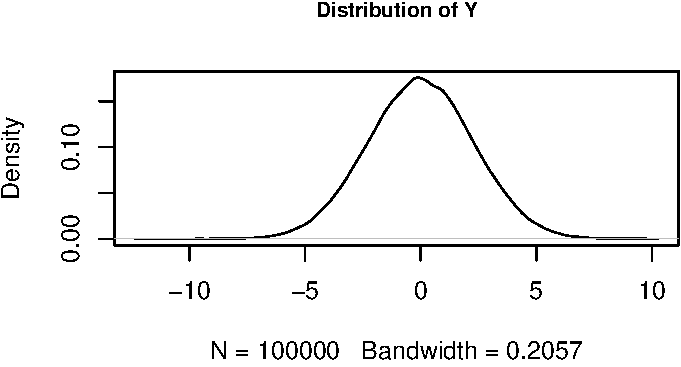
\includegraphics{applied_blp_sim_files/figure-latex/unnamed-chunk-2-1} 

}

\end{figure}

The individual predictive densities have partial access of the above set
of covariates. \(f_1\) has access to only \(X_0\) and \(X_1\), \(f_2\)
has access to only \(X_0\) and \(X_2\), and \(f_3\) has access to only
\(X_0\) and \(X_3\). We want to combine \(f_1,f_2,\) and \(f_3\) to
predict \(Y\). In this setup, \(X_0\) represent shared information,
while other covariates represent information unique to each individual
model.

We estimate the pooling/combination formulas on a random sample
\({(f_{1i} , f_{2i} , f_{3i}, Y_i) : i = 1,..., n}\) of size
\(n = 80,000\) and evaluate on an independent test sample of
\(n=20,000\). In this scenario, \(a_1 = a_2 = 1\) and \(a_3 = 1.1\), so
that \(f_3\) is a more concentrated, sharper density forecast than
\(f_1\) and \(f_2\) (Gneiting and Ranjan (2013)) and they are defined as
follows:

\[
\begin{aligned}
f_1&=\text{N}(X_0+a_1X_1,1+a^2_2+a^2_3)\\
f_2&=\text{N}(X_0+a_2X_2,1+a^2_1+a^2_3)\\
f_3&=\text{N}(X_0+a_3X_3,1+a^2_1+a^2_2)\\
\end{aligned}
\]

\begin{table}[H]
\caption{\label{tab:unnamed-chunk-5}Model and Beta Mixing Weight Parameters}

\centering
\fontsize{8}{10}\selectfont
\begin{tabular}[t]{lrrrrr}
\toprule
  & $\omega_1$ & $\omega_2$ & $\omega_3$ & $\alpha$ & $\beta$\\
\midrule
TLP & 0.252 & 0.276 & 0.473 & NA & NA\\
BLP & 0.287 & 0.304 & 0.410 & 1.454 & 1.451\\
EW & 0.333 & 0.333 & 0.333 & NA & NA\\
EW-BLP & 0.333 & 0.333 & 0.333 & 1.456 & 1.454\\
\bottomrule
\end{tabular}
\centering
\begin{tabular}[t]{lrrrrr}
\toprule
  & $w_1$ & $w_2$ & $w_3$ & $w_4$ & $w_5$\\
\midrule
BMC2 & 0.307 & 0.693 & NA & NA & NA\\
EW-BMC2 & 0.306 & 0.694 & NA & NA & NA\\
BMC3 & 0.042 & 0.605 & 0.353 & NA & NA\\
EW-BMC3 & 0.099 & 0.301 & 0.600 & NA & NA\\
BMC4 & 0.042 & 0.331 & 0.421 & 0.206 & NA\\
\addlinespace
EW-BMC4 & 0.101 & 0.300 & 0.397 & 0.202 & NA\\
BMC5 & 0.042 & 0.216 & 0.322 & 0.373 & 0.047\\
EW-BMC5 & 0.100 & 0.202 & 0.301 & 0.348 & 0.049\\
\bottomrule
\end{tabular}
\end{table}

\begin{table}[H]

\caption{\label{tab:unnamed-chunk-5}Mixture Parameters}
\centering
\fontsize{8}{10}\selectfont
\begin{tabular}[t]{lrrrrrrrrrr}
\toprule
  & $\alpha_1$ & $\beta_1$ & $\alpha_2$ & $\beta_2$ & $\alpha_3$ & $\beta_3$ & $\alpha_4$ & $\beta_4$ & $\alpha_5$ & $\beta_5$\\
\midrule
BMC2 & 1.190 & 1.172 & 1.617 & 1.625 & NA & NA & NA & NA & NA & NA\\
EW-BMC2 & 1.208 & 1.187 & 1.607 & 1.618 & NA & NA & NA & NA & NA & NA\\
BMC3 & 0.802 & 0.796 & 1.498 & 2.096 & 2.560 & 1.419 & NA & NA & NA & NA\\
EW-BMC3 & 1.213 & 1.153 & 1.258 & 1.260 & 1.647 & 1.658 & NA & NA & NA & NA\\
BMC4 & 0.802 & 0.787 & 1.441 & 1.534 & 1.743 & 1.424 & 1.418 & 1.937 & NA & NA\\
\addlinespace
EW-BMC4 & 1.272 & 1.176 & 1.335 & 1.397 & 1.767 & 1.765 & 1.297 & 1.257 & NA & NA\\
BMC5 & 0.803 & 0.788 & 1.469 & 1.421 & 2.411 & 1.507 & 1.492 & 2.312 & 1.443 & 1.280\\
EW-BMC5 & 1.291 & 1.190 & 1.329 & 1.295 & 1.357 & 1.460 & 1.807 & 1.780 & 1.223 & 1.129\\
\bottomrule
\end{tabular}
\end{table}

\begin{table}[H]

\caption{\label{tab:unnamed-chunk-5}Mixture Parameters}
\centering
\fontsize{8}{10}\selectfont
\begin{tabular}[t]{lrrrrrrrrrrrrrrr}
\toprule
  & $\omega_{11}$ & $\omega_{12}$ & $\omega_{13}$ & $\omega_{21}$ & $\omega_{22}$ & $\omega_{23}$ & $\omega_{31}$ & $\omega_{32}$ & $\omega_{33}$ & $\omega_{41}$ & $\omega_{42}$ & $\omega_{43}$ & $\omega_{51}$ & $\omega_{52}$ & $\omega_{53}$\\
\midrule
BMC2 & 0.261 & 0.261 & 0.477 & 0.297 & 0.320 & 0.383 & NA & NA & NA & NA & NA & NA & NA & NA & NA\\
EW-BMC2 & 0.333 & 0.333 & 0.333 & 0.333 & 0.333 & 0.333 & NA & NA & NA & NA & NA & NA & NA & NA & NA\\
BMC3 & 0.006 & 0.001 & 0.992 & 0.304 & 0.305 & 0.390 & 0.281 & 0.329 & 0.390 & NA & NA & NA & NA & NA & NA\\
EW-BMC3 & 0.333 & 0.333 & 0.333 & 0.333 & 0.333 & 0.333 & 0.333 & 0.333 & 0.333 & NA & NA & NA & NA & NA & NA\\
BMC4 & 0.006 & 0.001 & 0.993 & 0.301 & 0.308 & 0.390 & 0.278 & 0.331 & 0.390 & 0.323 & 0.287 & 0.390 & NA & NA & NA\\
\addlinespace
EW-BMC4 & 0.333 & 0.333 & 0.333 & 0.333 & 0.333 & 0.333 & 0.333 & 0.333 & 0.333 & 0.333 & 0.333 & 0.333 & NA & NA & NA\\
BMC5 & 0.005 & 0.001 & 0.994 & 0.302 & 0.311 & 0.387 & 0.278 & 0.328 & 0.394 & 0.309 & 0.299 & 0.392 & 0.292 & 0.345 & 0.362\\
EW-BMC5 & 0.333 & 0.333 & 0.333 & 0.333 & 0.333 & 0.333 & 0.333 & 0.333 & 0.333 & 0.333 & 0.333 & 0.333 & 0.333 & 0.333 & 0.333\\
\bottomrule
\end{tabular}
\end{table}

\begin{table}[H]
\caption{\label{tab:unnamed-chunk-5}Log Score}

\centering
\fontsize{8}{10}\selectfont
\begin{tabular}[t]{lrr}
\toprule
  & Training & Test\\
\midrule
TLP & -1.910 & -1.908\\
BLP & -1.869 & -1.866\\
EW & -1.913 & -1.911\\
EW-BLP & -1.871 & -1.868\\
\bottomrule
\end{tabular}
\centering
\begin{tabular}[t]{lrr}
\toprule
  & Training & Test\\
\midrule
BMC2 & -1.869 & -1.866\\
EW-BMC2 & -1.871 & -1.868\\
BMC3 & -1.869 & -1.866\\
EW-BMC3 & -1.871 & -1.868\\
BMC4 & -1.869 & -1.866\\
\addlinespace
EW-BMC4 & -1.871 & -1.868\\
BMC5 & -1.869 & -1.866\\
EW-BMC5 & -1.871 & -1.868\\
\bottomrule
\end{tabular}
\end{table}

\begin{figure}[h]

{\centering 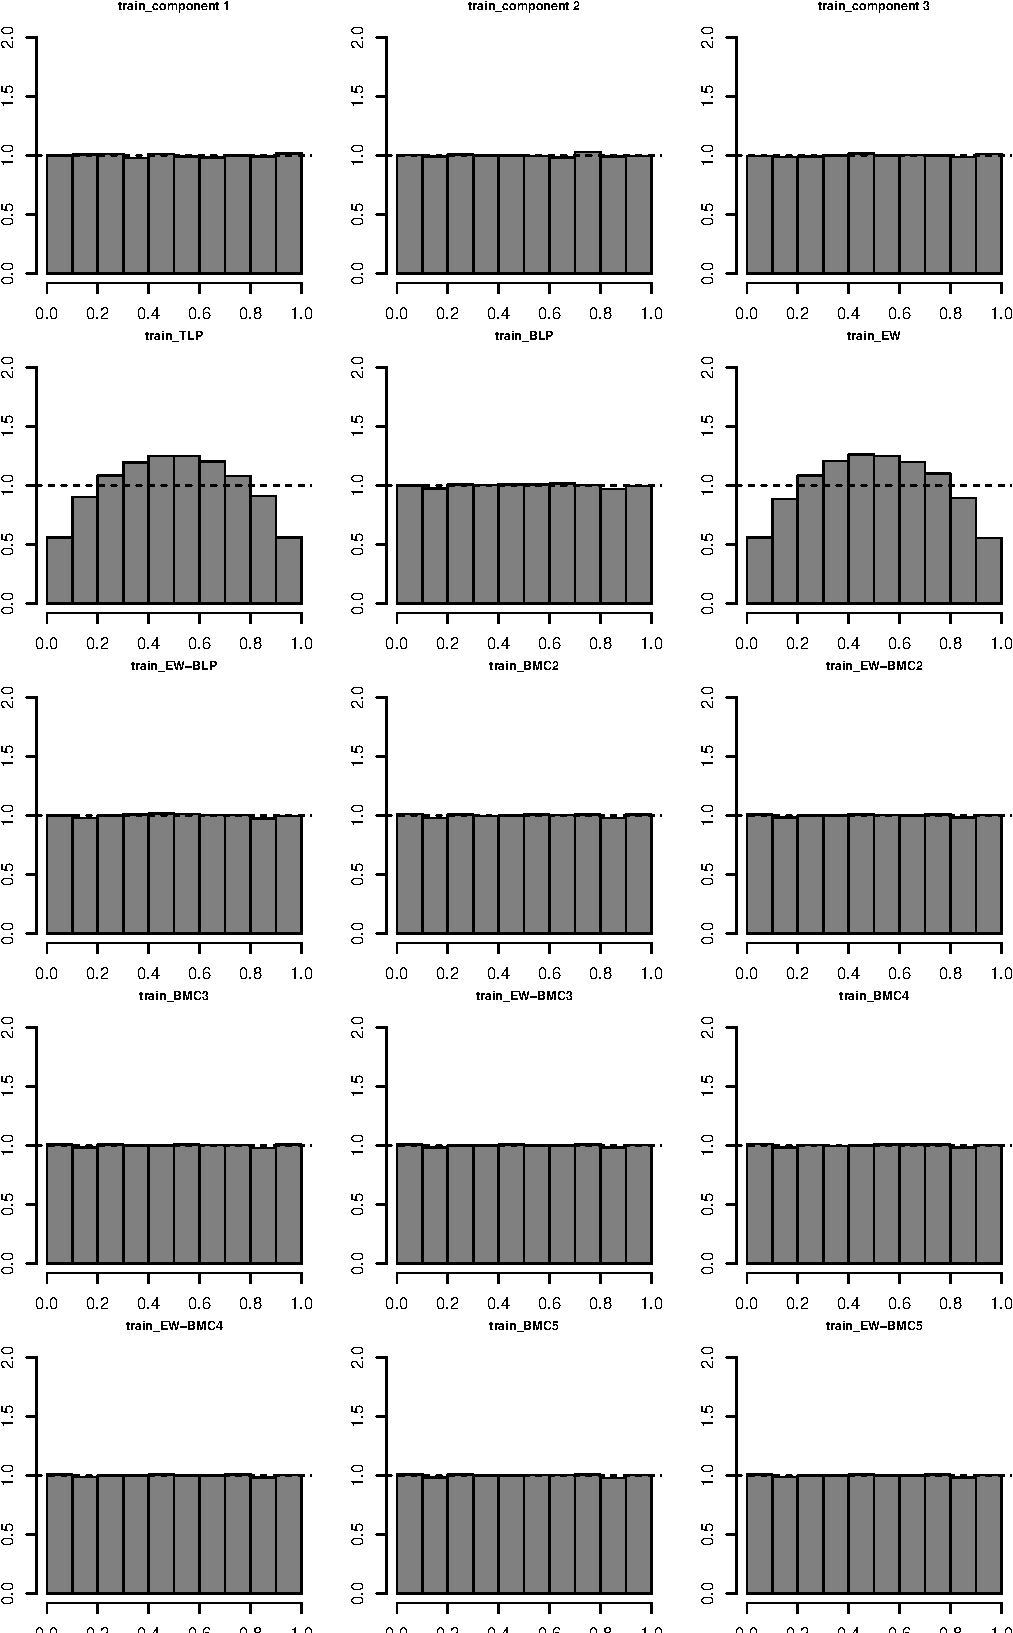
\includegraphics{applied_blp_sim_files/figure-latex/unnamed-chunk-6-1} 

}

\end{figure}

\clearpage

\begin{figure}[h]

{\centering 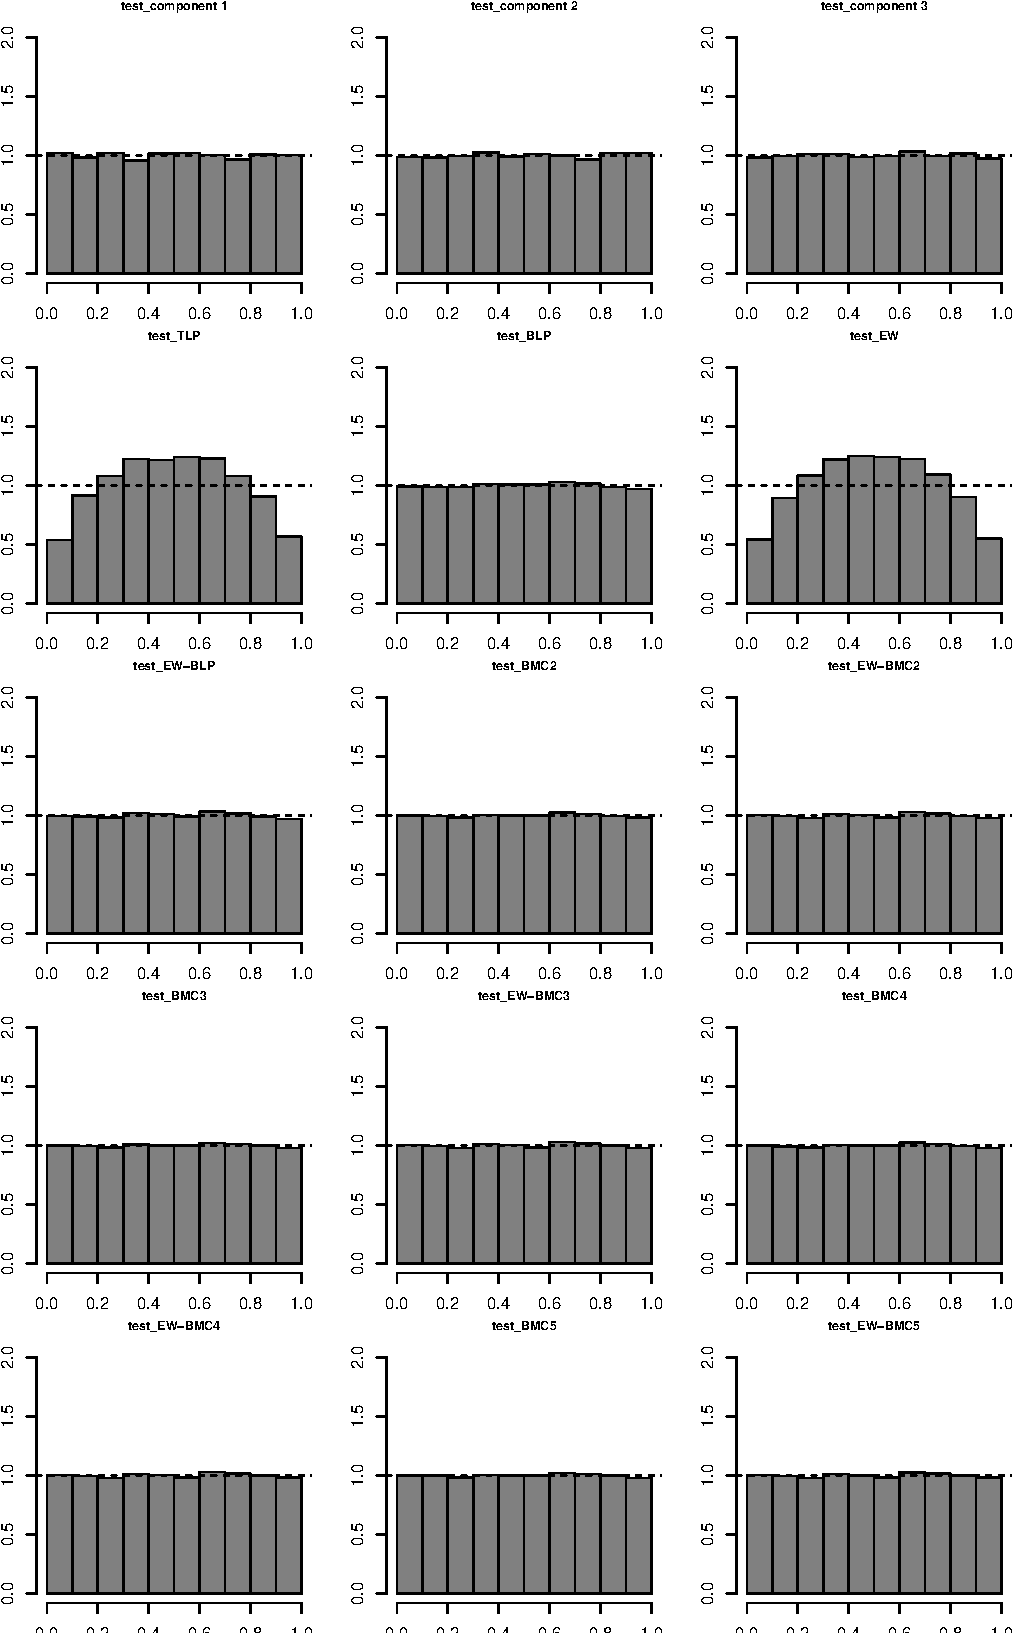
\includegraphics{applied_blp_sim_files/figure-latex/unnamed-chunk-7-1} 

}

\end{figure}

\clearpage

\hypertarget{scenario-2-multimodal-dgp-normal-mixture-and-close-mathcalm}{%
\subsection{\texorpdfstring{Scenario 2: Multimodal DGP (Normal mixture)
and
close-\(\mathcal{M}\)}{Scenario 2: Multimodal DGP (Normal mixture) and close-\textbackslash mathcal\{M\}}}\label{scenario-2-multimodal-dgp-normal-mixture-and-close-mathcalm}}

The data generating process for the observation \(y_t\) is

\[
y_t \overset{i.i.d.}{\sim} p_1\text{N}(-2,0.25)+p_2\text{N}(0,0.25)+p_3\text{N}(2,0.25), \\
t= 1,...,100,0000
\]

where \(p_1=0.2,p_2=0.2\), and \(p_3=0.6\). In this scenario, the three
component models are in the data generating process and the TLP's PITs
are approximately beta distributed (uniformly distributed,
specifically). This scenario serves to show the situation in which TLP
is an optimal method of combining forecast distributions. We expect BLP
and BMC to perform as equally well as TLP with higher complexity. In
other words, this is when BLP and BMC are not needed.

\begin{figure}[H]

{\centering 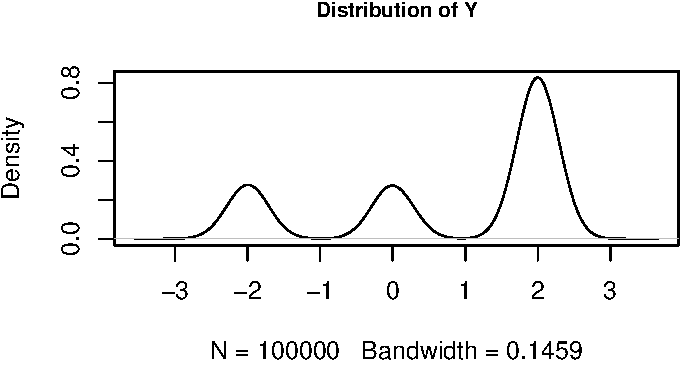
\includegraphics{applied_blp_sim_files/figure-latex/unnamed-chunk-9-1} 

}

\end{figure}

The individual predictive densities are defined as follows:

\[
\begin{aligned}
f_{1}&\overset{i.i.d.}{\sim}\text{N}(-2,0.25)\\
f_{2}&\overset{i.i.d.}{\sim}\text{N}(0,0.25)\\
f_{3}&\overset{i.i.d.}{\sim}\text{N}(2,0.25)\\
\end{aligned}
\]

\begin{table}[H]
\caption{\label{tab:unnamed-chunk-12}Model and Beta Mixing Weight Parameters}

\centering
\fontsize{8}{10}\selectfont
\begin{tabular}[t]{lrrrrr}
\toprule
  & $\omega_1$ & $\omega_2$ & $\omega_3$ & $\alpha$ & $\beta$\\
\midrule
TLP & 0.201 & 0.198 & 0.601 & NA & NA\\
BLP & 0.203 & 0.199 & 0.598 & 1.005 & 0.998\\
EW & 0.333 & 0.333 & 0.333 & NA & NA\\
EW-BLP & 0.333 & 0.333 & 0.333 & 1.246 & 0.785\\
\bottomrule
\end{tabular}
\centering
\begin{tabular}[t]{lrrrrr}
\toprule
  & $w_1$ & $w_2$ & $w_3$ & $w_4$ & $w_5$\\
\midrule
BMC2 & 0.300 & 0.700 & NA & NA & NA\\
EW-BMC2 & 0.284 & 0.716 & NA & NA & NA\\
BMC3 & 0.100 & 0.300 & 0.600 & NA & NA\\
EW-BMC3 & 0.395 & 0.457 & 0.149 & NA & NA\\
BMC4 & 0.097 & 0.300 & 0.402 & 0.201 & NA\\
\addlinespace
EW-BMC4 & 0.115 & 0.340 & 0.304 & 0.241 & NA\\
BMC5 & 0.099 & 0.200 & 0.310 & 0.342 & 0.049\\
EW-BMC5 & 0.122 & 0.251 & 0.271 & 0.304 & 0.051\\
\bottomrule
\end{tabular}
\end{table}

\begin{table}[H]

\caption{\label{tab:unnamed-chunk-12}Mixture Parameters}
\centering
\fontsize{8}{10}\selectfont
\begin{tabular}[t]{lrrrrrrrrrr}
\toprule
  & $\alpha_1$ & $\beta_1$ & $\alpha_2$ & $\beta_2$ & $\alpha_3$ & $\beta_3$ & $\alpha_4$ & $\beta_4$ & $\alpha_5$ & $\beta_5$\\
\midrule
BMC2 & 1.001 & 1.002 & 1.008 & 0.996 & NA & NA & NA & NA & NA & NA\\
EW-BMC2 & 1.153 & 3.075 & 4.263 & 1.223 & NA & NA & NA & NA & NA & NA\\
BMC3 & 1.000 & 0.999 & 1.004 & 0.999 & 1.007 & 0.997 & NA & NA & NA & NA\\
EW-BMC3 & 6.650 & 1.147 & 1.063 & 1.546 & 41.391 & 14.170 & NA & NA & NA & NA\\
BMC4 & 0.880 & 0.906 & 0.958 & 0.940 & 1.109 & 1.072 & 0.925 & 0.999 & NA & NA\\
\addlinespace
EW-BMC4 & 0.942 & 0.740 & 0.946 & 0.739 & 11.571 & 2.925 & 0.944 & 0.739 & NA & NA\\
BMC5 & 0.892 & 0.903 & 0.983 & 0.948 & 1.127 & 1.029 & 0.957 & 1.050 & 0.865 & 0.863\\
EW-BMC5 & 0.946 & 0.739 & 0.944 & 0.740 & 0.946 & 0.739 & 11.572 & 2.925 & 0.939 & 0.739\\
\bottomrule
\end{tabular}
\end{table}

\begin{table}[H]

\caption{\label{tab:unnamed-chunk-12}Mixture Parameters}
\centering
\fontsize{8}{10}\selectfont
\begin{tabular}[t]{lrrrrrrrrrrrrrrr}
\toprule
  & $\omega_{11}$ & $\omega_{12}$ & $\omega_{13}$ & $\omega_{21}$ & $\omega_{22}$ & $\omega_{23}$ & $\omega_{31}$ & $\omega_{32}$ & $\omega_{33}$ & $\omega_{41}$ & $\omega_{42}$ & $\omega_{43}$ & $\omega_{51}$ & $\omega_{52}$ & $\omega_{53}$\\
\midrule
BMC2 & 0.202 & 0.198 & 0.599 & 0.204 & 0.199 & 0.597 & NA & NA & NA & NA & NA & NA & NA & NA & NA\\
EW-BMC2 & 0.333 & 0.333 & 0.333 & 0.333 & 0.333 & 0.333 & NA & NA & NA & NA & NA & NA & NA & NA & NA\\
BMC3 & 0.203 & 0.198 & 0.599 & 0.205 & 0.199 & 0.596 & 0.203 & 0.198 & 0.599 & NA & NA & NA & NA & NA & NA\\
EW-BMC3 & 0.333 & 0.333 & 0.333 & 0.333 & 0.333 & 0.333 & 0.333 & 0.333 & 0.333 & NA & NA & NA & NA & NA & NA\\
BMC4 & 0.156 & 0.210 & 0.634 & 0.190 & 0.159 & 0.651 & 0.258 & 0.210 & 0.532 & 0.131 & 0.216 & 0.653 & NA & NA & NA\\
\addlinespace
EW-BMC4 & 0.333 & 0.333 & 0.333 & 0.333 & 0.333 & 0.333 & 0.333 & 0.333 & 0.333 & 0.333 & 0.333 & 0.333 & NA & NA & NA\\
BMC5 & 0.160 & 0.209 & 0.632 & 0.201 & 0.156 & 0.643 & 0.286 & 0.198 & 0.516 & 0.143 & 0.212 & 0.645 & 0.204 & 0.197 & 0.599\\
EW-BMC5 & 0.333 & 0.333 & 0.333 & 0.333 & 0.333 & 0.333 & 0.333 & 0.333 & 0.333 & 0.333 & 0.333 & 0.333 & 0.333 & 0.333 & 0.333\\
\bottomrule
\end{tabular}
\end{table}

\begin{table}[H]
\caption{\label{tab:unnamed-chunk-12}Log Score}

\centering
\fontsize{8}{10}\selectfont
\begin{tabular}[t]{lrr}
\toprule
  & Training & Test\\
\midrule
TLP & -0.983 & -0.981\\
BLP & -0.983 & -0.981\\
EW & -1.132 & -1.134\\
EW-BLP & -1.044 & -1.042\\
\bottomrule
\end{tabular}
\centering
\begin{tabular}[t]{lrr}
\toprule
  & Training & Test\\
\midrule
BMC2 & -0.983 & -0.981\\
EW-BMC2 & -1.006 & -1.002\\
BMC3 & -0.983 & -0.981\\
EW-BMC3 & -0.992 & -0.988\\
BMC4 & -0.983 & -0.981\\
\addlinespace
EW-BMC4 & -1.001 & -1.000\\
BMC5 & -0.983 & -0.981\\
EW-BMC5 & -1.001 & -1.000\\
\bottomrule
\end{tabular}
\end{table}

\clearpage

\begin{figure}[h]

{\centering 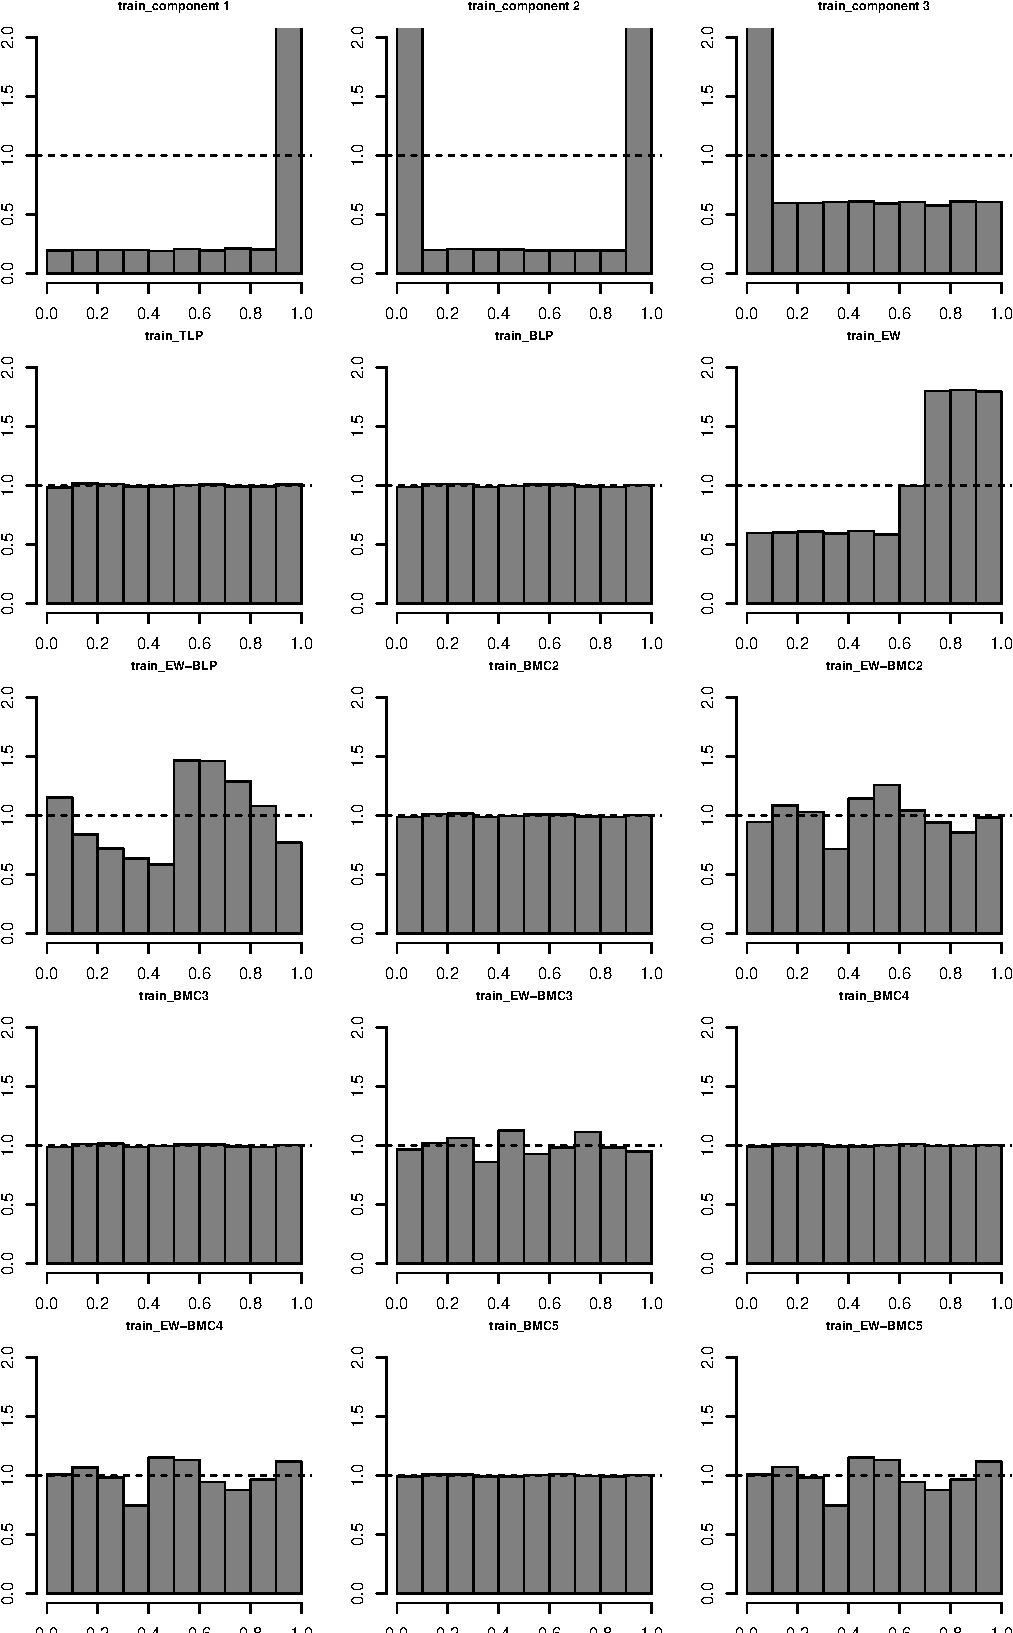
\includegraphics{applied_blp_sim_files/figure-latex/unnamed-chunk-13-1} 

}

\end{figure}

\clearpage

\begin{figure}[h]

{\centering 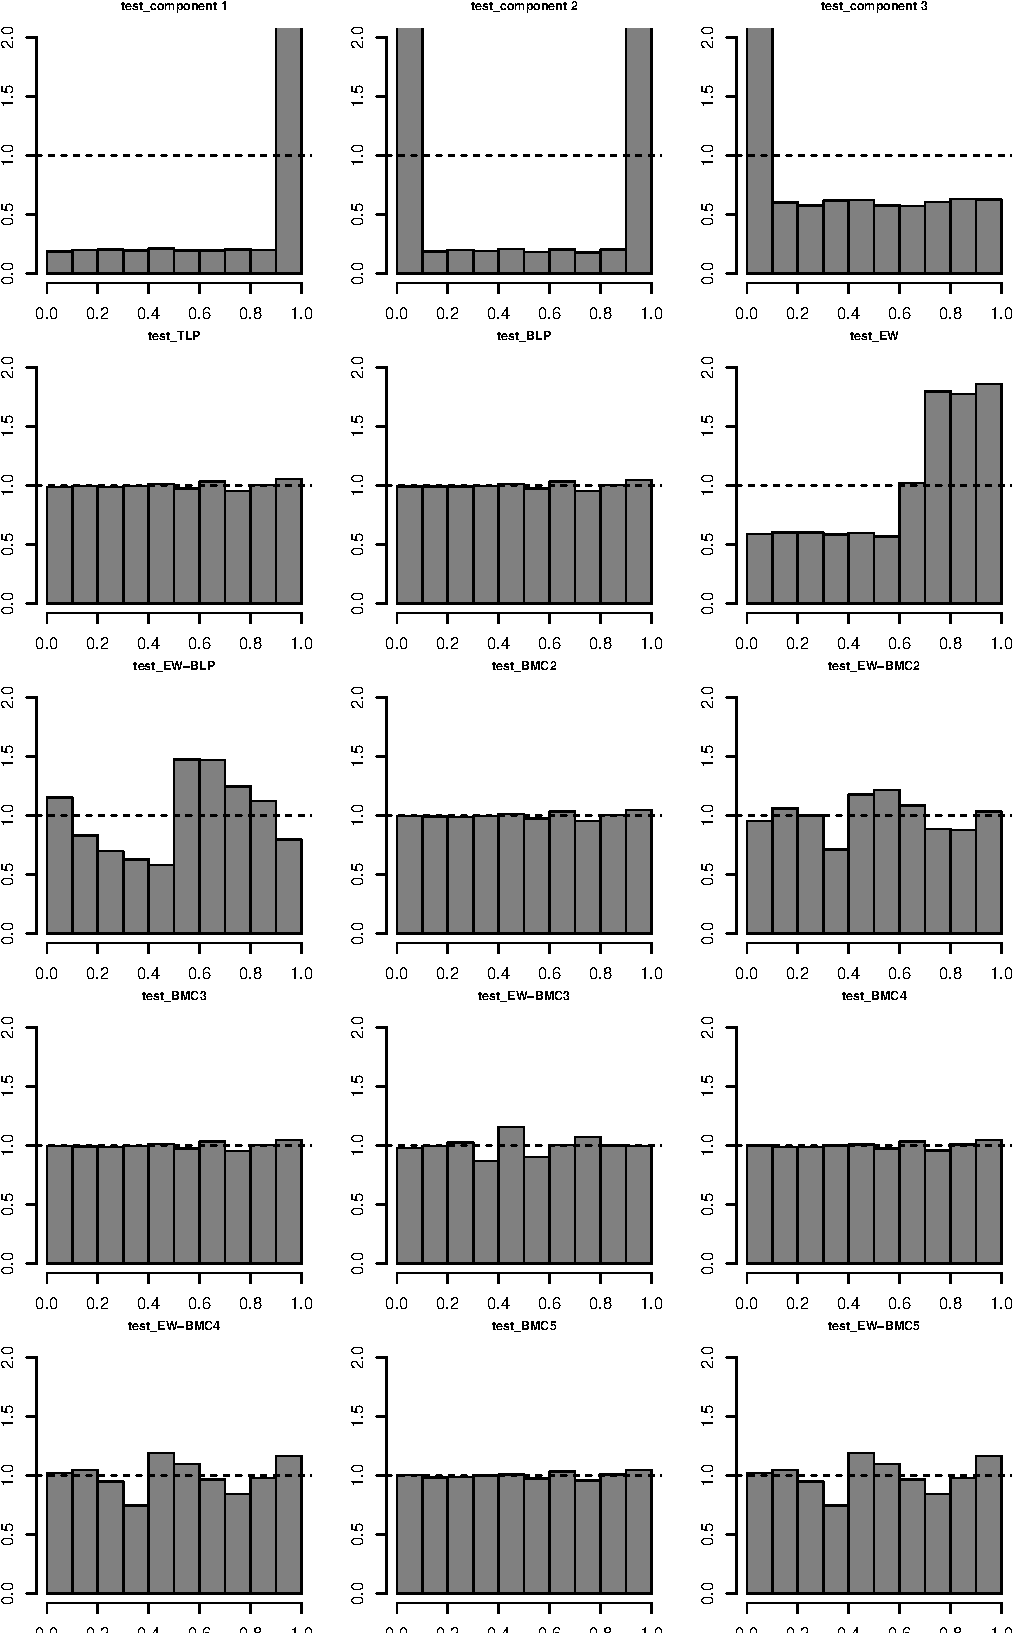
\includegraphics{applied_blp_sim_files/figure-latex/unnamed-chunk-14-1} 

}

\end{figure}

\clearpage

\begin{figure}[h]

{\centering 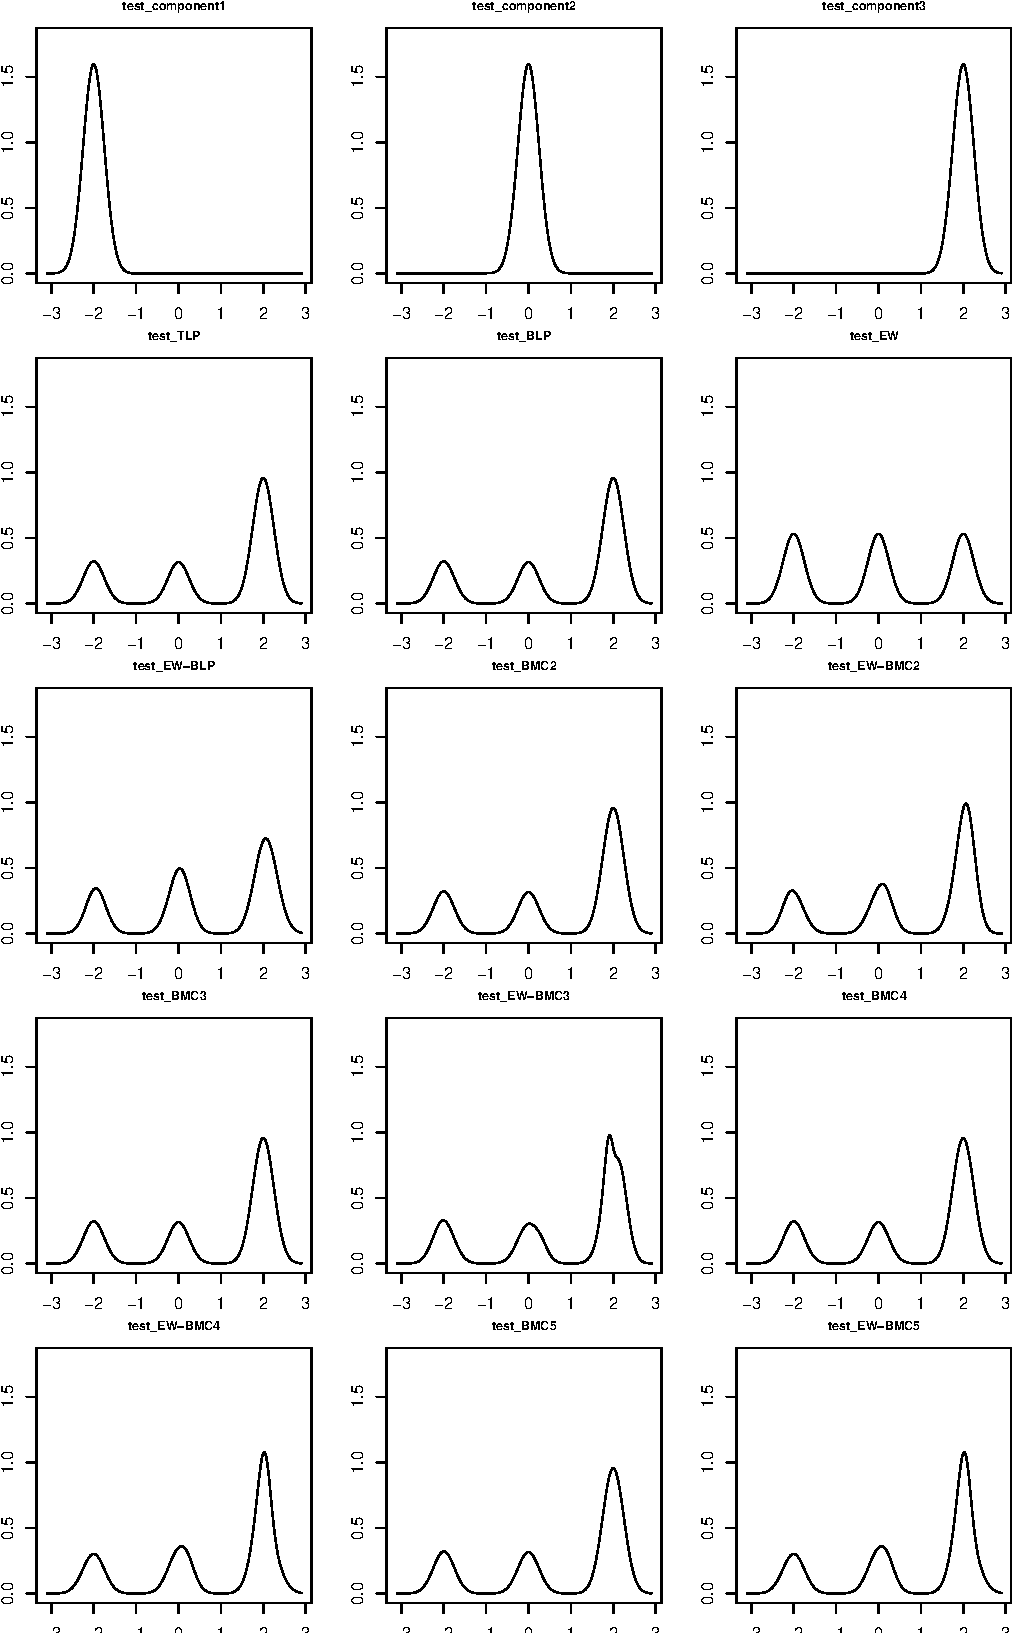
\includegraphics{applied_blp_sim_files/figure-latex/unnamed-chunk-15-1} 

}

\end{figure}

\clearpage

\hypertarget{scenario-3-multimodal-dgp-normal-mixture-and-open-mathcalm}{%
\subsection{\texorpdfstring{Scenario 3: Multimodal DGP (Normal mixture)
and
open-\(\mathcal{M}\)}{Scenario 3: Multimodal DGP (Normal mixture) and open-\textbackslash mathcal\{M\}}}\label{scenario-3-multimodal-dgp-normal-mixture-and-open-mathcalm}}

The data generating process for the observations in this scenario is the
same as in Scenario 2. There are two component models defined as follows

\[
\begin{aligned}
f_{1}&\overset{i.i.d.}{\sim}\text{N}(2,1)\\
f_{2}&\overset{i.i.d.}{\sim}\text{N}(-1,1).\\
\end{aligned}
\]

The component models are not part of the data generating process. In
this scenario the TLP's PITs are not approximately beta distributed, so
we expect BLP to not be able to find optimal \(\alpha\) and \(\beta\) to
calibrate the PITs. Specifically, this scenario serves to motivate BMC
and show that BMC is highly flexible and can calibrate the PITs when BLP
cannot. We also expect BMC with higher K to be more flexible than BMC
with lower K.

\begin{table}[H]
\caption{\label{tab:unnamed-chunk-18}Model and Beta Mixing Weight Parameters}

\centering
\fontsize{8}{10}\selectfont
\begin{tabular}[t]{lrrrr}
\toprule
  & $\omega_1$ & $\omega_2$ & $\alpha$ & $\beta$\\
\midrule
TLP & 0.660 & 0.340 & NA & NA\\
BLP & 0.782 & 0.218 & 1.038 & 1.638\\
EW & 0.500 & 0.500 & NA & NA\\
EW-BLP & 0.500 & 0.500 & 1.391 & 1.285\\
\bottomrule
\end{tabular}
\centering
\begin{tabular}[t]{lrrrrr}
\toprule
  & $w_1$ & $w_2$ & $w_3$ & $w_4$ & $w_5$\\
\midrule
BMC2 & 0.399 & 0.601 & NA & NA & NA\\
EW-BMC2 & 0.201 & 0.799 & NA & NA & NA\\
BMC3 & 0.000 & 0.601 & 0.399 & NA & NA\\
EW-BMC3 & 0.133 & 0.305 & 0.562 & NA & NA\\
BMC4 & 0.080 & 0.601 & 0.118 & 0.201 & NA\\
\addlinespace
EW-BMC4 & 0.001 & 0.197 & 0.601 & 0.201 & NA\\
BMC5 & NA & NA & NA & NA & NA\\
EW-BMC5 & 0.601 & 0.201 & NA & NA & NA\\
\bottomrule
\end{tabular}
\end{table}

\begin{table}[H]

\caption{\label{tab:unnamed-chunk-18}Mixture Parameters}
\centering
\fontsize{8}{10}\selectfont
\begin{tabular}[t]{lrrrrrrrrrr}
\toprule
  & $\alpha_1$ & $\beta_1$ & $\alpha_2$ & $\beta_2$ & $\alpha_3$ & $\beta_3$ & $\alpha_4$ & $\beta_4$ & $\alpha_5$ & $\beta_5$\\
\midrule
BMC2 & 0.954 & 31.846 & 12.802 & 12.791 & NA & NA & NA & NA & NA & NA\\
EW-BMC2 & 6.804 & 75.092 & 7.260 & 3.637 & NA & NA & NA & NA & NA & NA\\
BMC3 & 0.000 & 0.000 & 12.803 & 12.791 & 0.954 & 31.849 & NA & NA & NA & NA\\
EW-BMC3 & 1.121 & 2.656 & 1.121 & 2.659 & 63.118 & 20.933 & NA & NA & NA & NA\\
BMC4 & 3.610 & 100.703 & 12.732 & 12.728 & 4.129 & 199.463 & 6.663 & 69.664 & NA & NA\\
\addlinespace
EW-BMC4 & 3.952 & 9.582 & 76.843 & 101.783 & 55.935 & 18.728 & 6.736 & 74.176 & NA & NA\\
BMC5 & 0.881 & 24.579 & 101.811 & 101.781 & 1.548 & 74.779 & 0.087 & 0.913 & 104.313 & -103.313\\
EW-BMC5 & 52.160 & 126.465 & 32.119 & 42.544 & 60.617 & 20.295 & 0.000 & 0.001 & 2.672 & -2.475\\
\bottomrule
\end{tabular}
\end{table}

\begin{table}[H]

\caption{\label{tab:unnamed-chunk-18}Mixture Parameters}
\centering
\fontsize{8}{10}\selectfont
\begin{tabular}[t]{lrrrrrrrrrr}
\toprule
  & $\omega_{11}$ & $\omega_{12}$ & $\omega_{21}$ & $\omega_{22}$ & $\omega_{31}$ & $\omega_{32}$ & $\omega_{41}$ & $\omega_{42}$ & $\omega_{51}$ & $\omega_{52}$\\
\midrule
BMC2 & 0.967 & 0.033 & 1.000 & 0.00 & NA & NA & NA & NA & NA & NA\\
EW-BMC2 & 0.500 & 0.500 & 0.500 & 0.50 & NA & NA & NA & NA & NA & NA\\
BMC3 & 0.987 & 0.013 & 1.000 & 0.00 & 0.967 & 0.033 & NA & NA & NA & NA\\
EW-BMC3 & 0.500 & 0.500 & 0.500 & 0.50 & 0.500 & 0.500 & NA & NA & NA & NA\\
BMC4 & 1.000 & 0.000 & 1.000 & 0.00 & 1.000 & 0.000 & 0.476 & 0.524 & NA & NA\\
\addlinespace
EW-BMC4 & 0.500 & 0.500 & 0.500 & 0.50 & 0.500 & 0.500 & 0.500 & 0.500 & NA & NA\\
BMC5 & 1.000 & 0.524 & 0.476 & 0.08 & 0.000 & 0.601 & 0.000 & 0.118 & 0.0 & 0.201\\
EW-BMC5 & 0.500 & 0.500 & 0.500 & 0.50 & 0.500 & 0.500 & 0.500 & 0.500 & 0.5 & 0.500\\
\bottomrule
\end{tabular}
\end{table}

\begin{table}[H]
\caption{\label{tab:unnamed-chunk-18}Log Score}

\centering
\fontsize{8}{10}\selectfont
\begin{tabular}[t]{lrr}
\toprule
  & Training & Test\\
\midrule
TLP & -1.742 & -1.739\\
BLP & -1.679 & -1.676\\
EW & -1.785 & -1.784\\
EW-BLP & -1.757 & -1.755\\
\bottomrule
\end{tabular}
\centering
\begin{tabular}[t]{lrr}
\toprule
  & Training & Test\\
\midrule
BMC2 & -1.208 & -1.204\\
EW-BMC2 & -1.385 & -1.380\\
BMC3 & -1.208 & -1.204\\
EW-BMC3 & -1.292 & -1.287\\
BMC4 & -0.983 & -0.982\\
\addlinespace
EW-BMC4 & -0.987 & -0.986\\
BMC5 & -0.983 & -0.982\\
EW-BMC5 & -1.287 & -1.283\\
\bottomrule
\end{tabular}
\end{table}

\clearpage

\begin{figure}[h]

{\centering 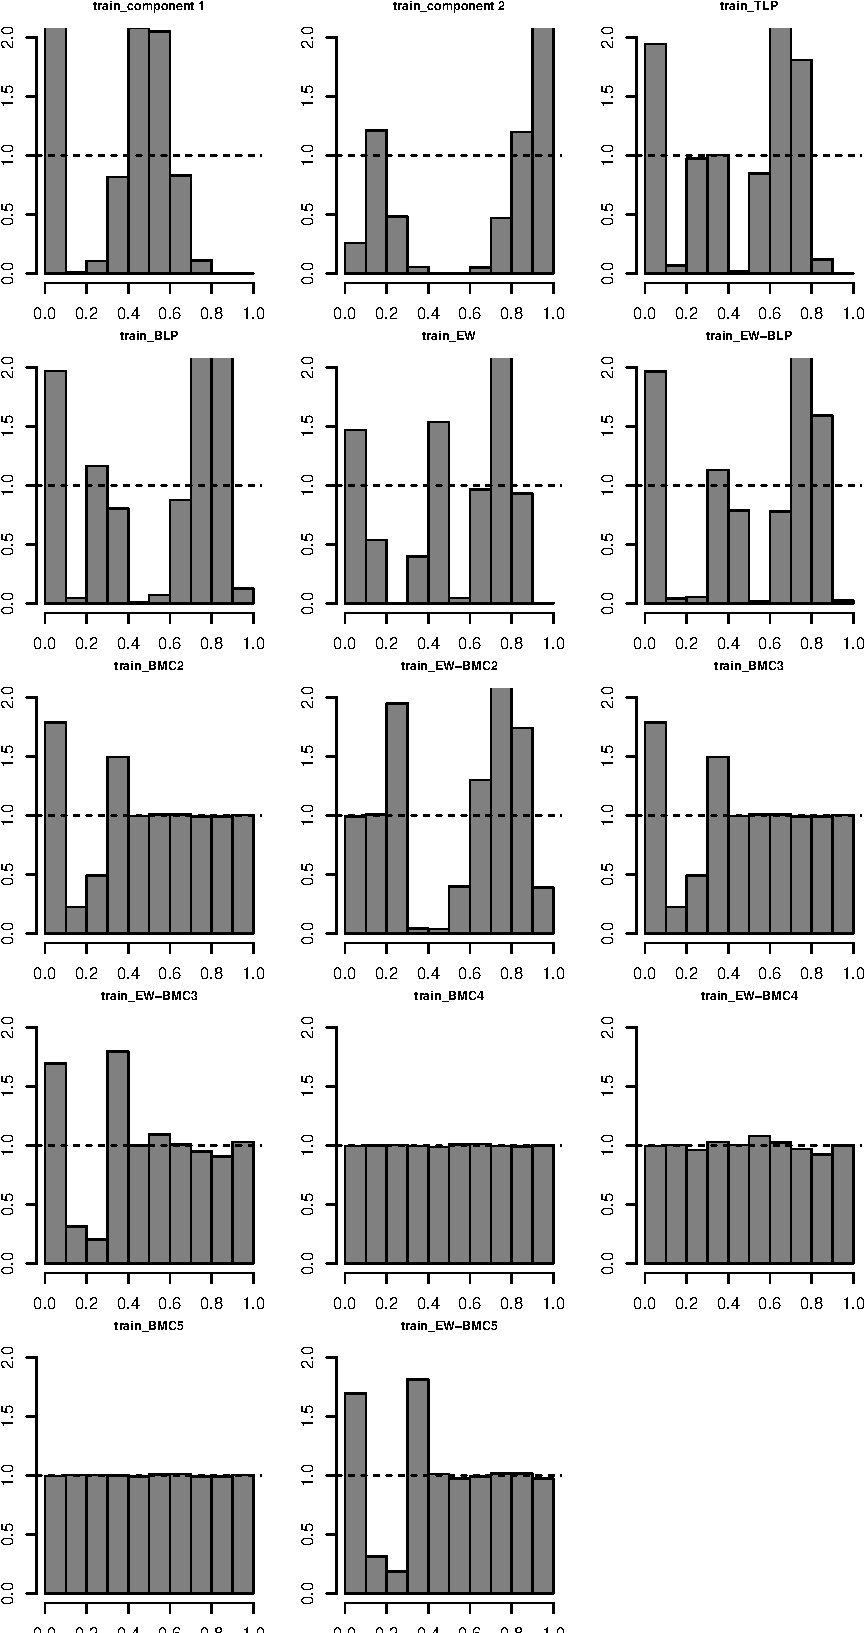
\includegraphics{applied_blp_sim_files/figure-latex/unnamed-chunk-19-1} 

}

\end{figure}

\clearpage

\begin{figure}[h]

{\centering 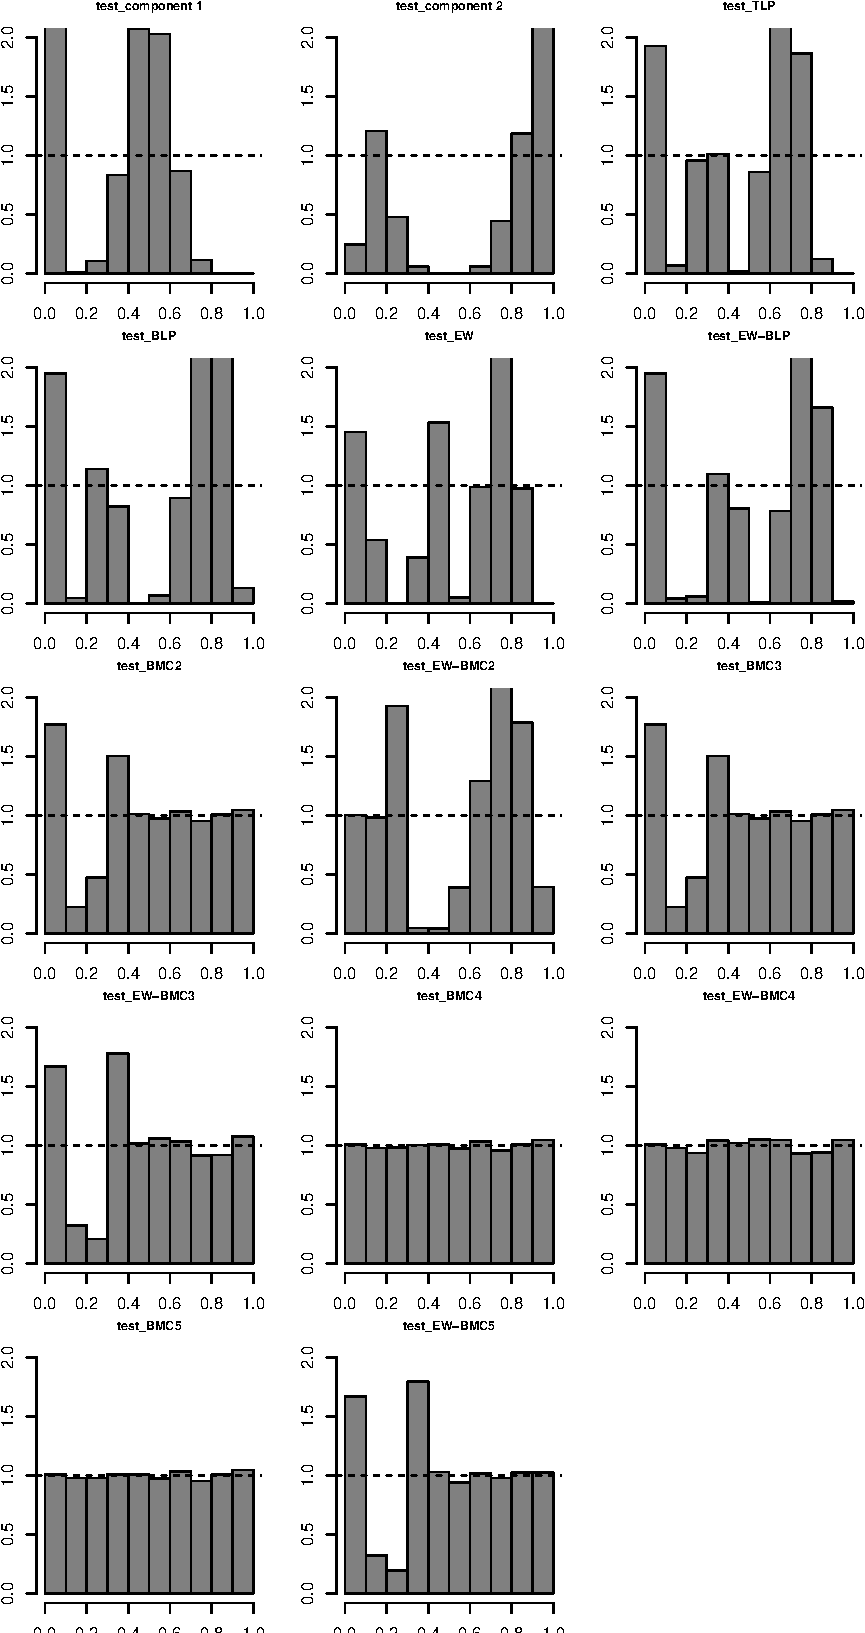
\includegraphics{applied_blp_sim_files/figure-latex/unnamed-chunk-20-1} 

}

\end{figure}

\clearpage

\begin{figure}[h]

{\centering 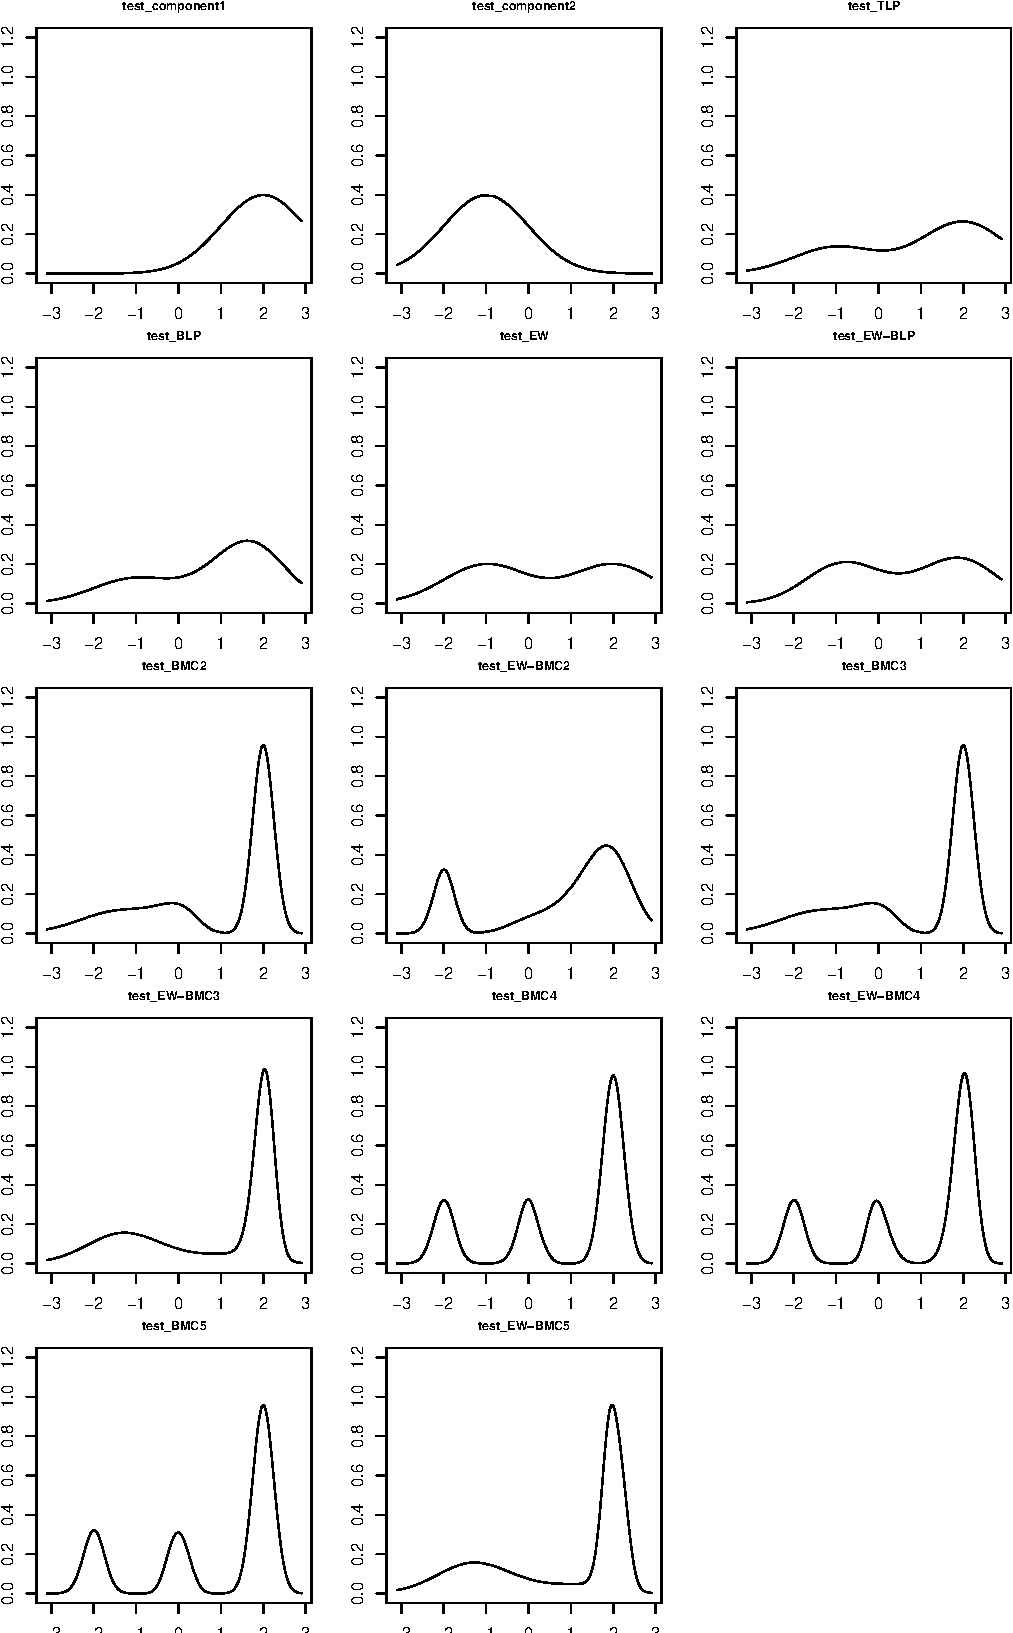
\includegraphics{applied_blp_sim_files/figure-latex/unnamed-chunk-21-1} 

}

\end{figure}

\end{document}
